\section{Introduction}

\begin{figure}[htbp]
	\centerline{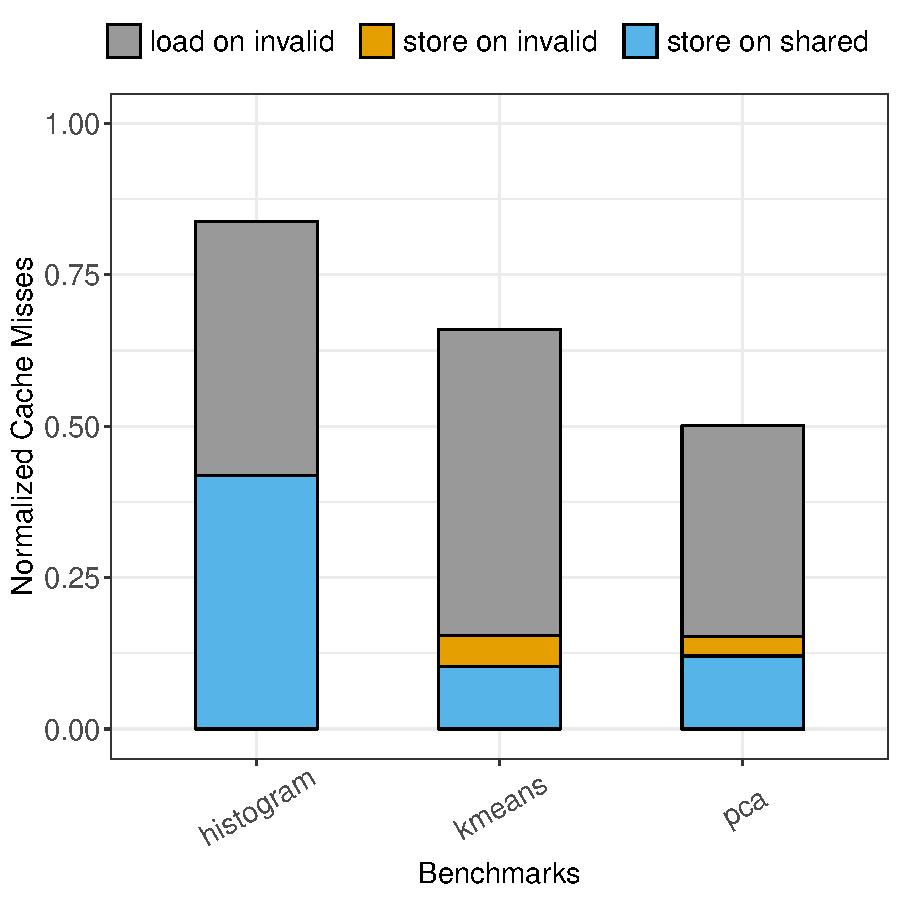
\includegraphics[scale=0.5]{graphs/normalized_cache_misses.pdf}}
	\caption{Breakdown of L1-d cache misses due to coherence states, i.e., invalid or read-only (shared). All other misses are due to lines not being in cache.}
\label{fig:coherence_misses}
\end{figure}

% -- Introduction part

Uni-core processor scaling over that past decade has stagnated due to increasing power consumption for marginal performance gains. Modern computing systems are seeing proliferation into multi-core and many-core processors. Parallel and shared memory applications are becoming increasingly important to fully utilize these current and upcoming architectures. However, the communication bandwidth between compute units is the main bottleneck for further boosts in performance. The key to future advancements lies within the communication infrastructure, specifically the on-chip networks (NoCs) connecting cores and memories. NoC traffic congestion stems from intensive memory accesses issued from the on-chip cores \cite{Wang2008}, and with multiple cores using a shared memory model, theses accesses are largely made of cache coherence traffic.

%  -- Motivation goes here

% Points to discuss
% \begin{enumerate}
% 	\item Traffic on NoCs come memory requests
% 	\item Many of the memory requests are due to misses on shared memory, coherence misses
% 	\item refer to Figure 1
% 	\item Out of these misses, many of them are from coherence, at least 50\% from the kernels we observed
% 	\item Misses on stores make up a non-trivial portion of the coherence misses
% 	\item Many misses from silent stores, pointing to inherent value locality (refer to some values of silent store percentage from other papers)
% 	\item Look into domain of approximate computing
% 	\item instead of just value locality (exact silent stores), programs can be error toleratant. So we look at value similarity, specifically store-value similarity
% 	\item Using store value similarity we can determine estimate performance to output quality tradoffs. For example with a narrow distribution (most of the store misses store similar values, so if we approximate within those bounds we can save a lot of store misses. However for a wide distribution it means that the stores store vastly differing values so you might not be able to save a lot of misses by using a narrow approximation band. The output quality may also suffer)
% 	\item not much has been done in terms of approximation in coherence protocols, (refer approx loads on CMPs - but on loads not stores)
% 	\item we also introduce a coherence optimization to save on these store misses
% 	\item summarize with bullet points of contributions
% \end{enumerate}

Memory access misses private caches are either due to the cache line not being present or in the wrong coherence states. In a write-invalidate cache coherence protocol, a store operation to a local cache which misses for any reason would send invalidation requests to remote caches with the same cache line. Subsequent load or stores in the remote caches to that line would register a miss and generate corresponding coherence requests, i.e., traffic in the NoC. Figure \ref{fig:coherence_misses} shows a breakdown of L1-d cache misses normalized to the total amount of cache misses, on three benchmarks (Described in Section \ref{sec:benchmarks}). At least 50\% of the misses are due to being in the wrong coherence states, i.e., loads and stores on coherence invalidated lines, or stores on read-only (shared) lines. All other misses are due to the line not being present in the cache. In our preliminary findings, a substantial portion of misses are on loads due to invalidates caused by stores (put average number here), with a non-trivial portion of the coherence misses are on stores (put in average number here). 

A significant portion misses due to coherence related invalidation come from silent stores \cite{Lepak2002}, storing values that exactly match what is being overwitten. This suggest that there is a high degree of value locality \cite{Lipasti1996}. Existing work has examined squashing silent stores for reduce misses and improve performance \cite{Lepak2000, Lepak2002}. We however delve into the domain of approximate computing to expolit the intrinsic error-tolerance of certain applications to minimize coherence traffic with "acceptable" loss in application output quality. We do so by first introducting a novel workload characterization metric -- \textit{store-value similarity}. \textit{Store-value similarity} describes a probability distribution of the relative difference of a store value, and the value being overwritten in a memory location. It can be used to classify which applications would benefit from computing on approximate values to trade off output quality with a reduction in NoC traffic. Higher \textit{store-value similarity} corresponds to a higher probabilty of stores overwriting a memory location with values in a narrower range. Next we propose a coherence protocol optimization, Silent Approximate Stores (\textit{SAS}) tailored for error-tolerant, approximate applications to reduce coherence traffic by exploiting stores with high \textit{store-value similarity}. The protocol implements \textit{approximate stores}, where if the relative difference between a store value and what is being overwritten is within a programmer defined tolerance, the store is completed maintaining the lines current coherence state. This minimizes coherence traffic by inhibiting invalidations to remote caches which in turn reduces the amount of misses on subsequent accesses to invalidated lines.



To summerize, our work contributes two novel ideas from the approximate computing paradigm to exploit inherent error-tolerance in applications amenable to approximation.
\begin{itemize}
	\item We define a new characterization for approximate applications -- \textit{store-value similarity}, a metric to estimate the influence of approximations in computation to the reduction of coherence traffic.
	\item We propose a coherence optimization, Silent Approximate Stores (\textit{SAS}) to reduce coherence traffic in NoCs.	
\end{itemize}

Our preliminary implementation shows... TODO after evaluation, put some data here...